% The next command tells RStudio to do "Compile PDF" on book.Rnw,
% instead of this chapter, thereby eliminating the need to switch back to book.Rnw 
% before making the book.
%!TEX root = ../../book.Rnw

%blankpage

\chapter*{Author biographies}
\markboth{AUTHOR BIOGRAPHIES}{AUTHOR BIOGRAPHIES}
\addcontentsline{toc}{chapter}{\protect\numberline{}{Author biographies}}


\section*{Jeremy Van Antwerp}

% Adjust spacing so the photo looks nice in the paragraph.
\setlength{\intextsep}{-7pt}%
\setlength{\columnsep}{8pt}%
\begin{wrapfigure}{L}{0.25\textwidth}
  \begin{center}
    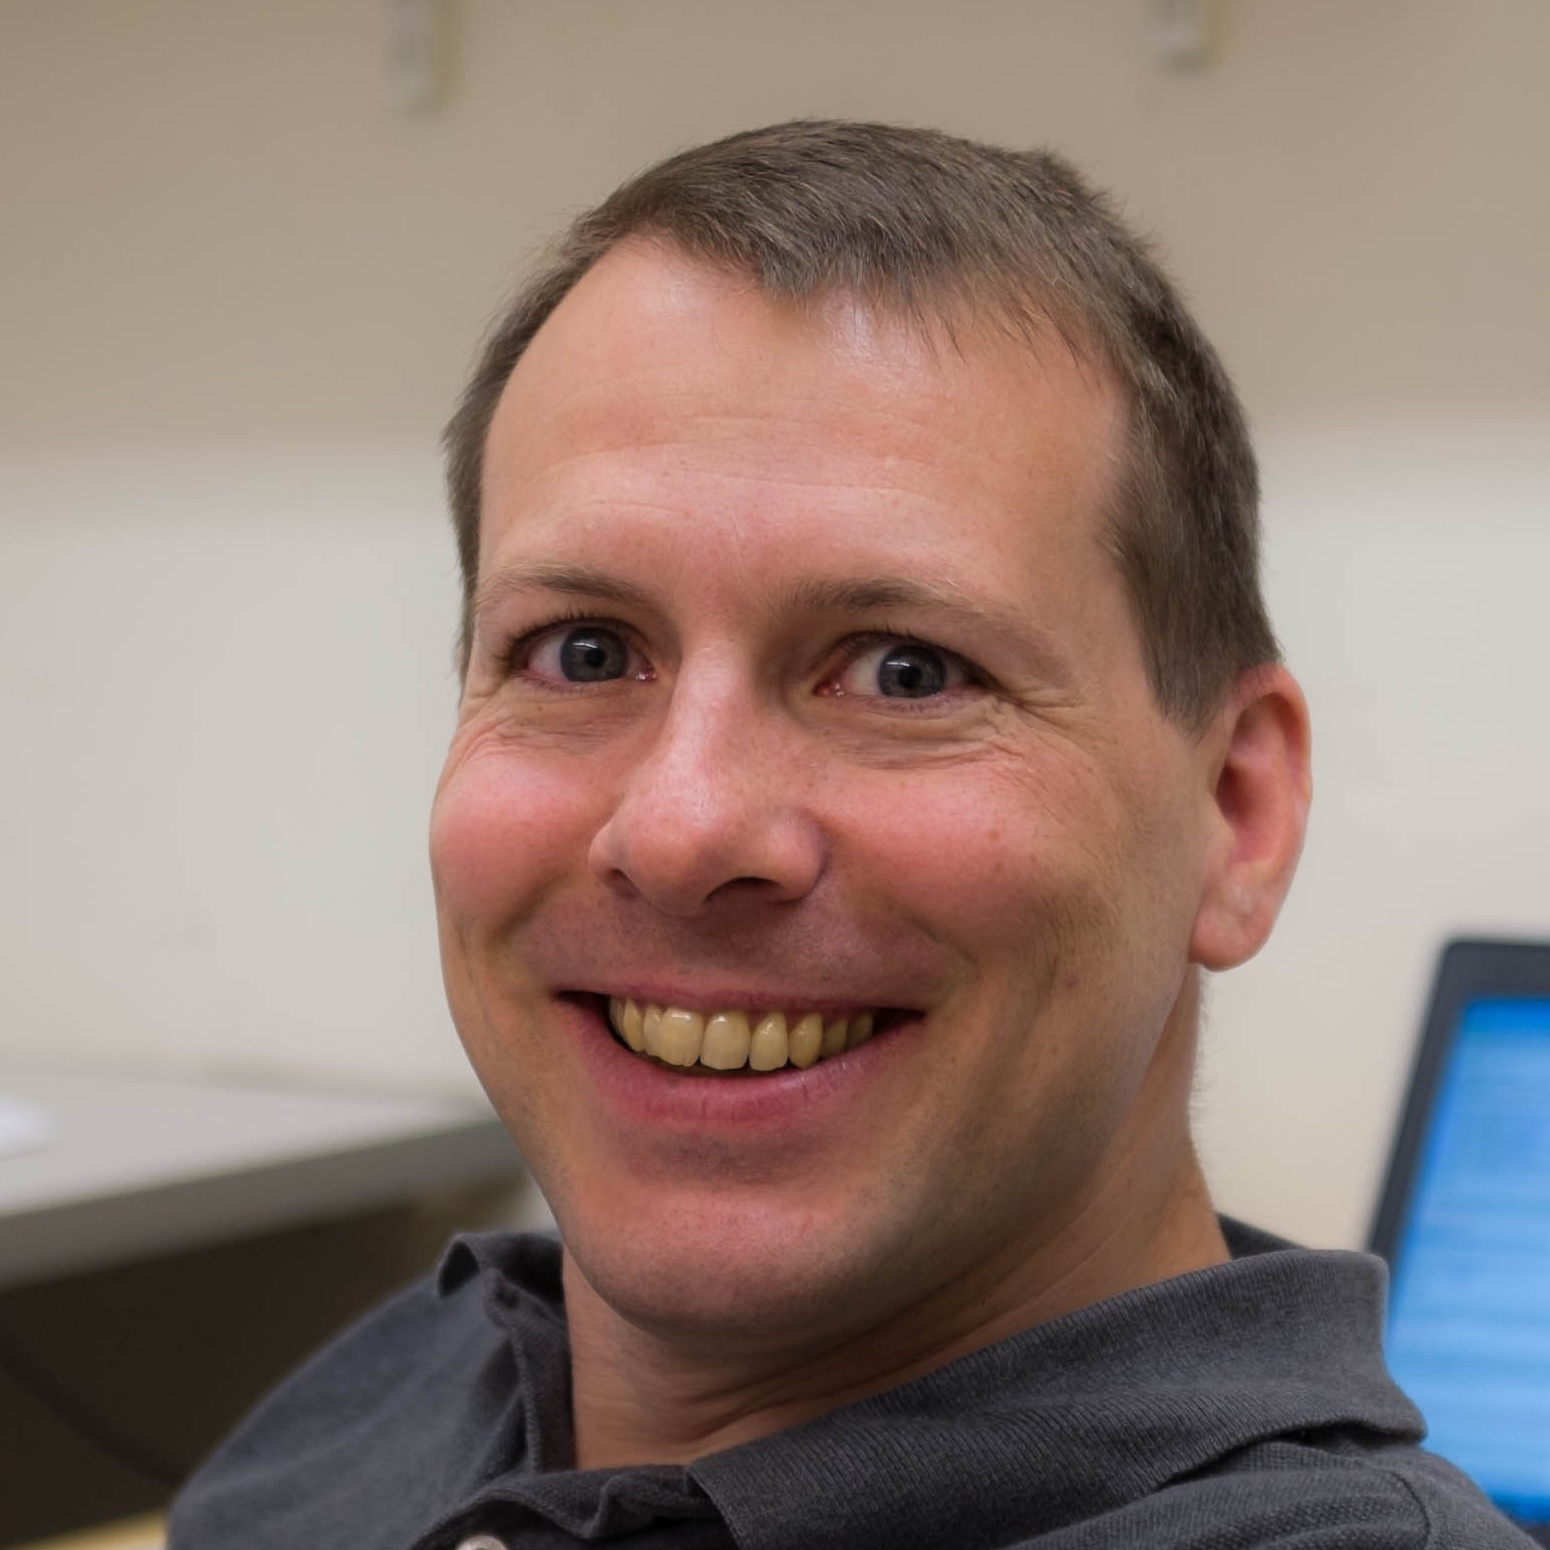
\includegraphics[width=0.25\textwidth]{headshots/jva-headshot.jpeg}
  \end{center}
\end{wrapfigure}
\textbf{Jeremy Van Antwerp} earned an M.S.\ and Ph.D.\ in chemical engineering 
from the University of Illinois at Urbana-Champaign. 
He is Professor of Engineering (chemical concentration)
at Calvin University in Grand Rapids, MI, USA
and has been a research affiliate and visiting scholar at the Massachusetts 
Institute of Technology, a journal editor, and a consultant in the pharmaceutical 
industry.
His research area is systems and process control.
He holds one US patent and is the author of \emph{Identifcation and control of 
sheet and film processes}~\cite{FeaVB2000}.
His poetry, cartoons, and puzzles have appeared in \emph{IEEE Control Systems}.
He is passionate about excellence and high-impact practices in education.
In 2001 he was awarded a Michigan Traditional Arts apprenticeship grant.


\section*{Matthew Kuperus Heun}

% Adjust spacing so the photo looks nice in the paragraph.
\setlength{\intextsep}{-7pt}%
\setlength{\columnsep}{8pt}%
\begin{wrapfigure}{L}{0.25\textwidth}
  \begin{center}
    \includegraphics[width=0.25\textwidth]{headshots/Heun_headshot}
  \end{center}
\end{wrapfigure}
\textbf{Matthew Kuperus Heun} is Professor of Engineering 
(mechanical concentration)
at Calvin University in Grand Rapids, MI, USA.
He earned an M.S.\ and Ph.D.\ in mechanical engineering from 
the University of Illinois at Urbana-Champaign and 
later worked at NASA's Jet Propulsion Laboratory and at Global Aerospace Corporation. 
He has been a visiting scholar at the Centre for Renewable and Sustainable Energy Studies 
at the University of Stellenbosch, South Africa. 
His long-term research question is 
``What is the relationship between energy and the economy when viewed through the lens of sustainability?''
In addition to scores of articles, he is lead author of 
\emph{Beyond GDP: National accounting in the age of resource depletion}~\citep{Heun:2015aa} 
and a co-editor of
\emph{Beyond Stewardship: New approaches to creation care}~\citep{Warners:2019aa}.


\bibliographystyle{unsrtnat}
\bibliography{MCBook2021}

